\documentclass{standalone}
\usepackage{tikz}
\usetikzlibrary{shapes}
\begin{document}

\pagestyle{empty}

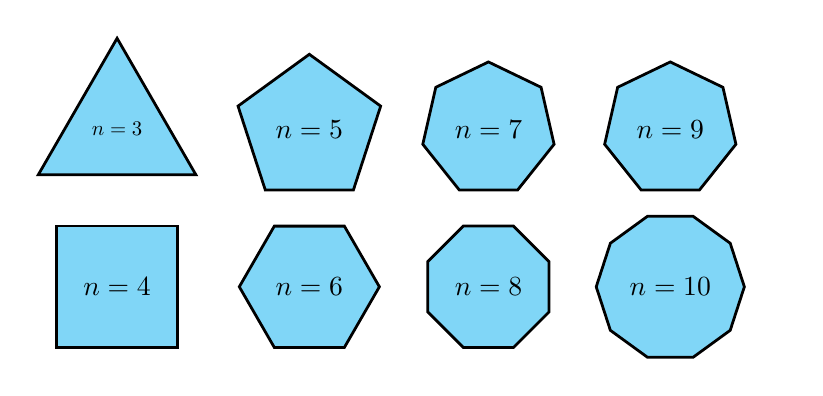
\begin{tikzpicture}[scale=2]
    \tikzstyle{ann} = [draw=none,fill=none,align=center]
    
    \matrix[nodes={draw, line width=1pt, fill=cyan!50},
        row sep=0.3cm,column sep=0.5cm] {
    %\node[ann, text width=2cm]{Regular \\ polygons}; &
    \node[regular polygon,regular polygon sides=3, scale=0.75, transform shape] {$n=3$};&
    \node[regular polygon,regular polygon sides=5] {$n=5$};&
    \node[regular polygon,regular polygon sides=7] {$n=7$};&
    \node[regular polygon,regular polygon sides=7] {$n=9$};&
    \\
    %\node[ann]{Stars};&
    \node[regular polygon,regular polygon sides=4] {$n=4$};&
    \node[regular polygon,regular polygon sides=6] {$n=6$};&
    \node[regular polygon,regular polygon sides=8] {$n=8$};&    
    \node[regular polygon,regular polygon sides=10] {$n=10$};
    \\
    };
\end{tikzpicture}


\end{document}
